\section{Preamp test}
This section will test all requirements on the \gls{preamp} 


\subsection{\autoref{req:preamp1}}
According to \autoref{req:preamp1}, a test was made to ensure that the \gls{preamp} not change the signal amplitude more than $\pm$\SI{1}{\decibel} between 20 Hz and 20 kHz. A test was made and is descried in \autoref{app:preamp_frequency_response} and the result is as following \autoref{fig:tests:appendix:amplitude}

\begin{figure}[htbp!]
	\centering
		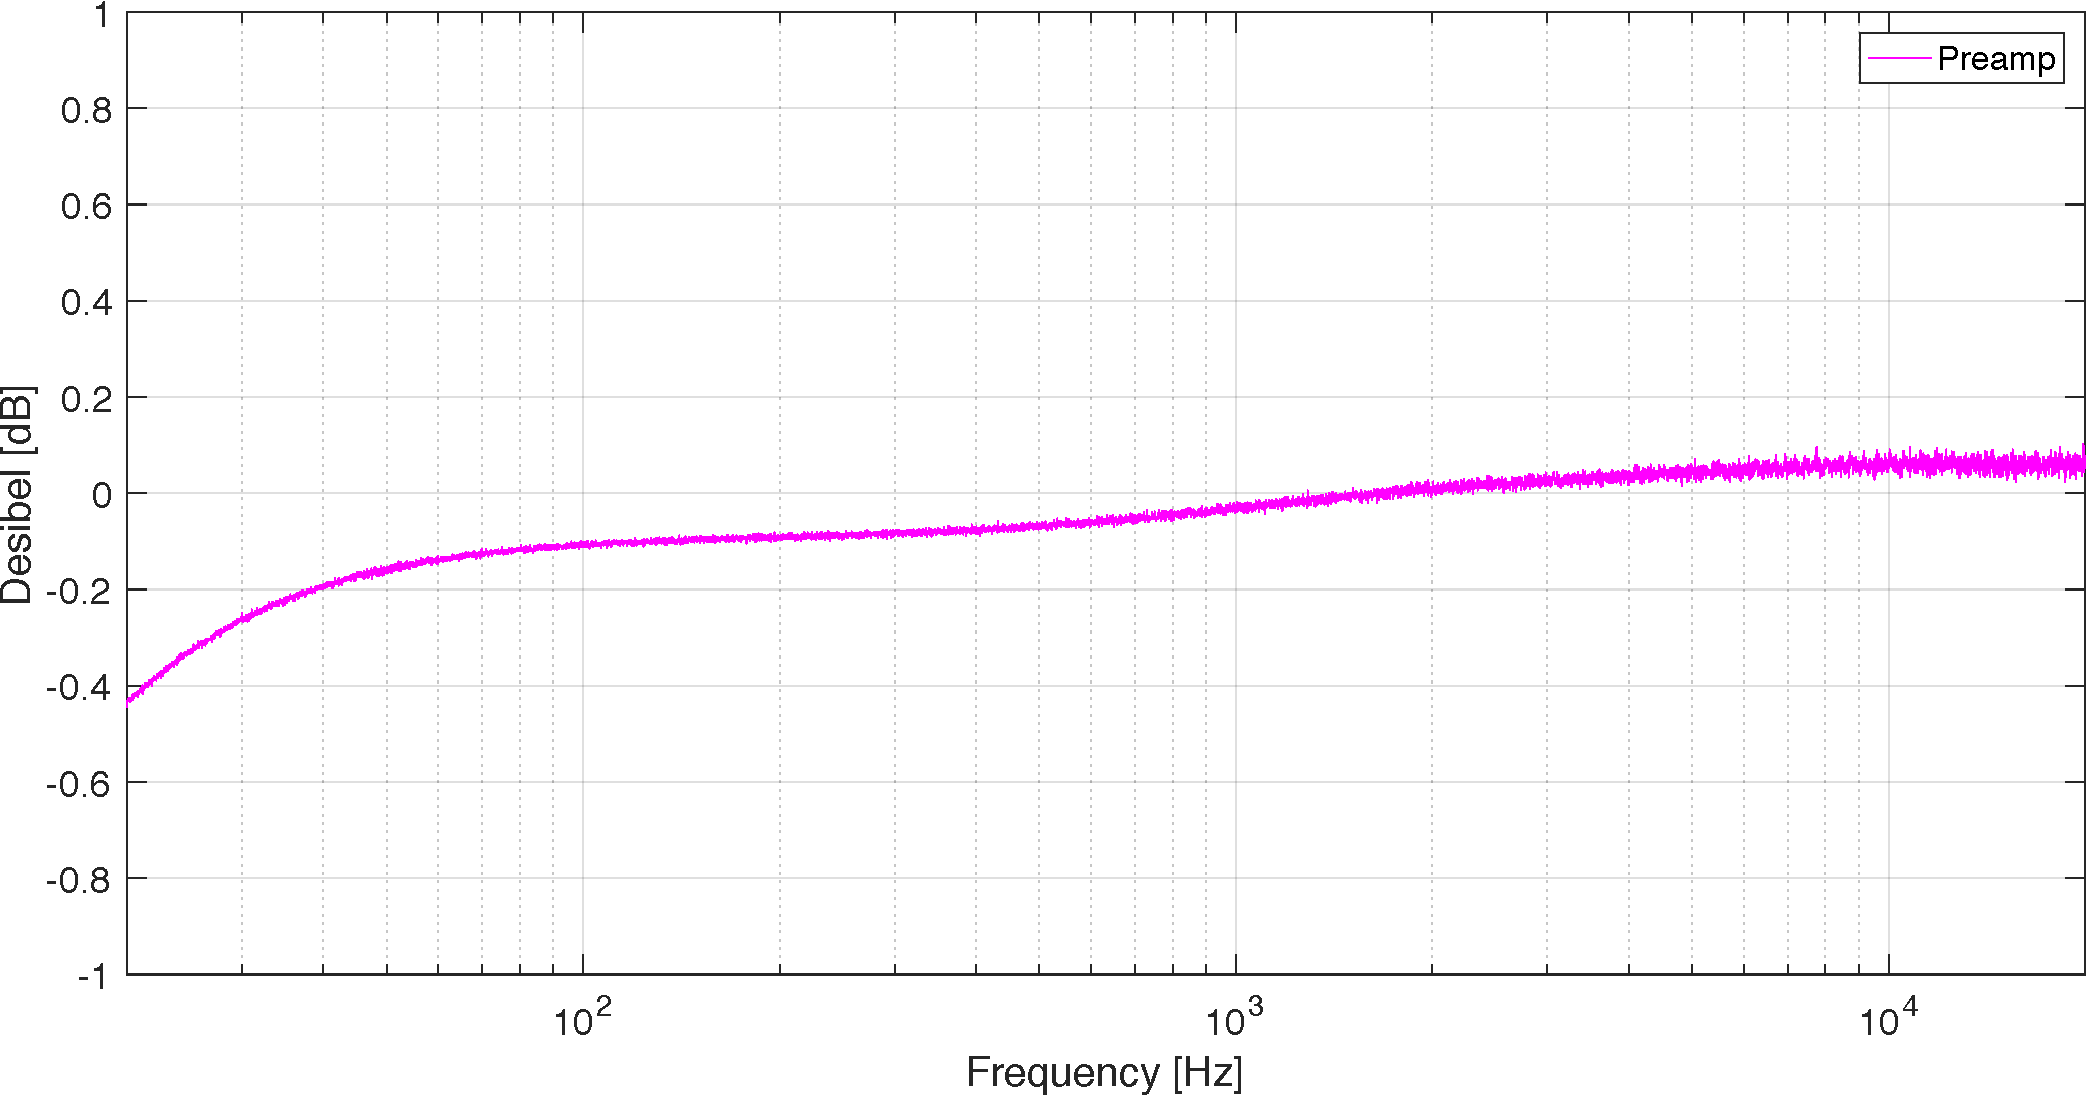
\includegraphics[width=1\textwidth]{preamp_frequency_responce.pdf}
		\caption{Measurement of the real output impedance of the three pickup settings.}
		\label{fig:tests:appendix:amplitude}
\end{figure}

The amplitude is within $\pm$\SI{1}{\decibel} so \autoref{req:preamp1} is approved


\subsection{\autoref{req:preamp2}}
According to \autoref{req:preamp2}, a test was made to ensure that the \gls{preamp} have an input impedance 10 times more than the highest output impedance of the guitar. According to \autoref{app:output_impedance} and the requirements the \gls{preamp} shall have an input impedance of at least \SI{730.8}{\kilo\ohm}. To ensure that the input impedance is over \SI{730.8}{\mega\ohm}, the input impedance of the \gls{opamp} is measured, and the result is to \SI{9.18}{\mega\ohm} according to \autoref{app:opamp_impedance}. Applying the input impedance to the following \autoref{eq:tests:preamp_result}, where $A$ is at least \SI{70}{\decibel}, according to ??  

\begin{equation}\label{eq:tests:preamp_result}
        Z_{In_{G1}} = R_{Bias} \parallel ((Z_i + Z_{i \beta}) \cdot (1+\beta \cdot A)) \simeq R_{Bias}
        \addunit{\si{\ohm}}
    \end{equation}

where the value from \autoref{label_Pre-amplifier} is applied as following \autoref{eq:tests:preamp_result_value}




\begin{subequations}\label{eq:tests:preamp_result_value}
\begin{equation}
        Z_{In_{G1}} = \SI{1}{\mega\ohm} \parallel ((\SI{9.18}{\mega\ohm} + 2550 \ohm) \cdot (1+ 0.5 \cdot 3162)) \simeq R_{Bias}
        \addunit{\si{\ohm}}
    \end{equation}
\centering
$\Updownarrow$
\begin{equation}
        Z_{In_{G1}} = \SI{1}{\mega\ohm} \parallel \SI{14.53}{\giga\ohm}  \simeq R_{Bias}
        \addunit{\si{\ohm}}
    \end{equation}
    $\Updownarrow$
\begin{equation}
        \SI{999.9}{\kilo\ohm} = \SI{1}{\mega\ohm} \parallel \SI{14.53}{\giga\ohm} 
        \addunit{\si{\ohm}}
    \end{equation}
 \end{subequations}

The calculated input impedance is higher than the required input impedance, so \autoref{req:preamp2} is approved


\subsection{\autoref{req:preamp5} and \autoref{req:preamp6}}
According to \autoref{req:preamp6}, a test was made to ensure that the \gls{preamp} \gls{pcb} including cable mound fits intro the Jack connector house. The first \autoref{fig:tests:preamp_pcb} shows the \gls{pcb} mounded on the jack connector and the cable is mounted on the \gls{preamp}

\begin{figure}[h]
	\centering
		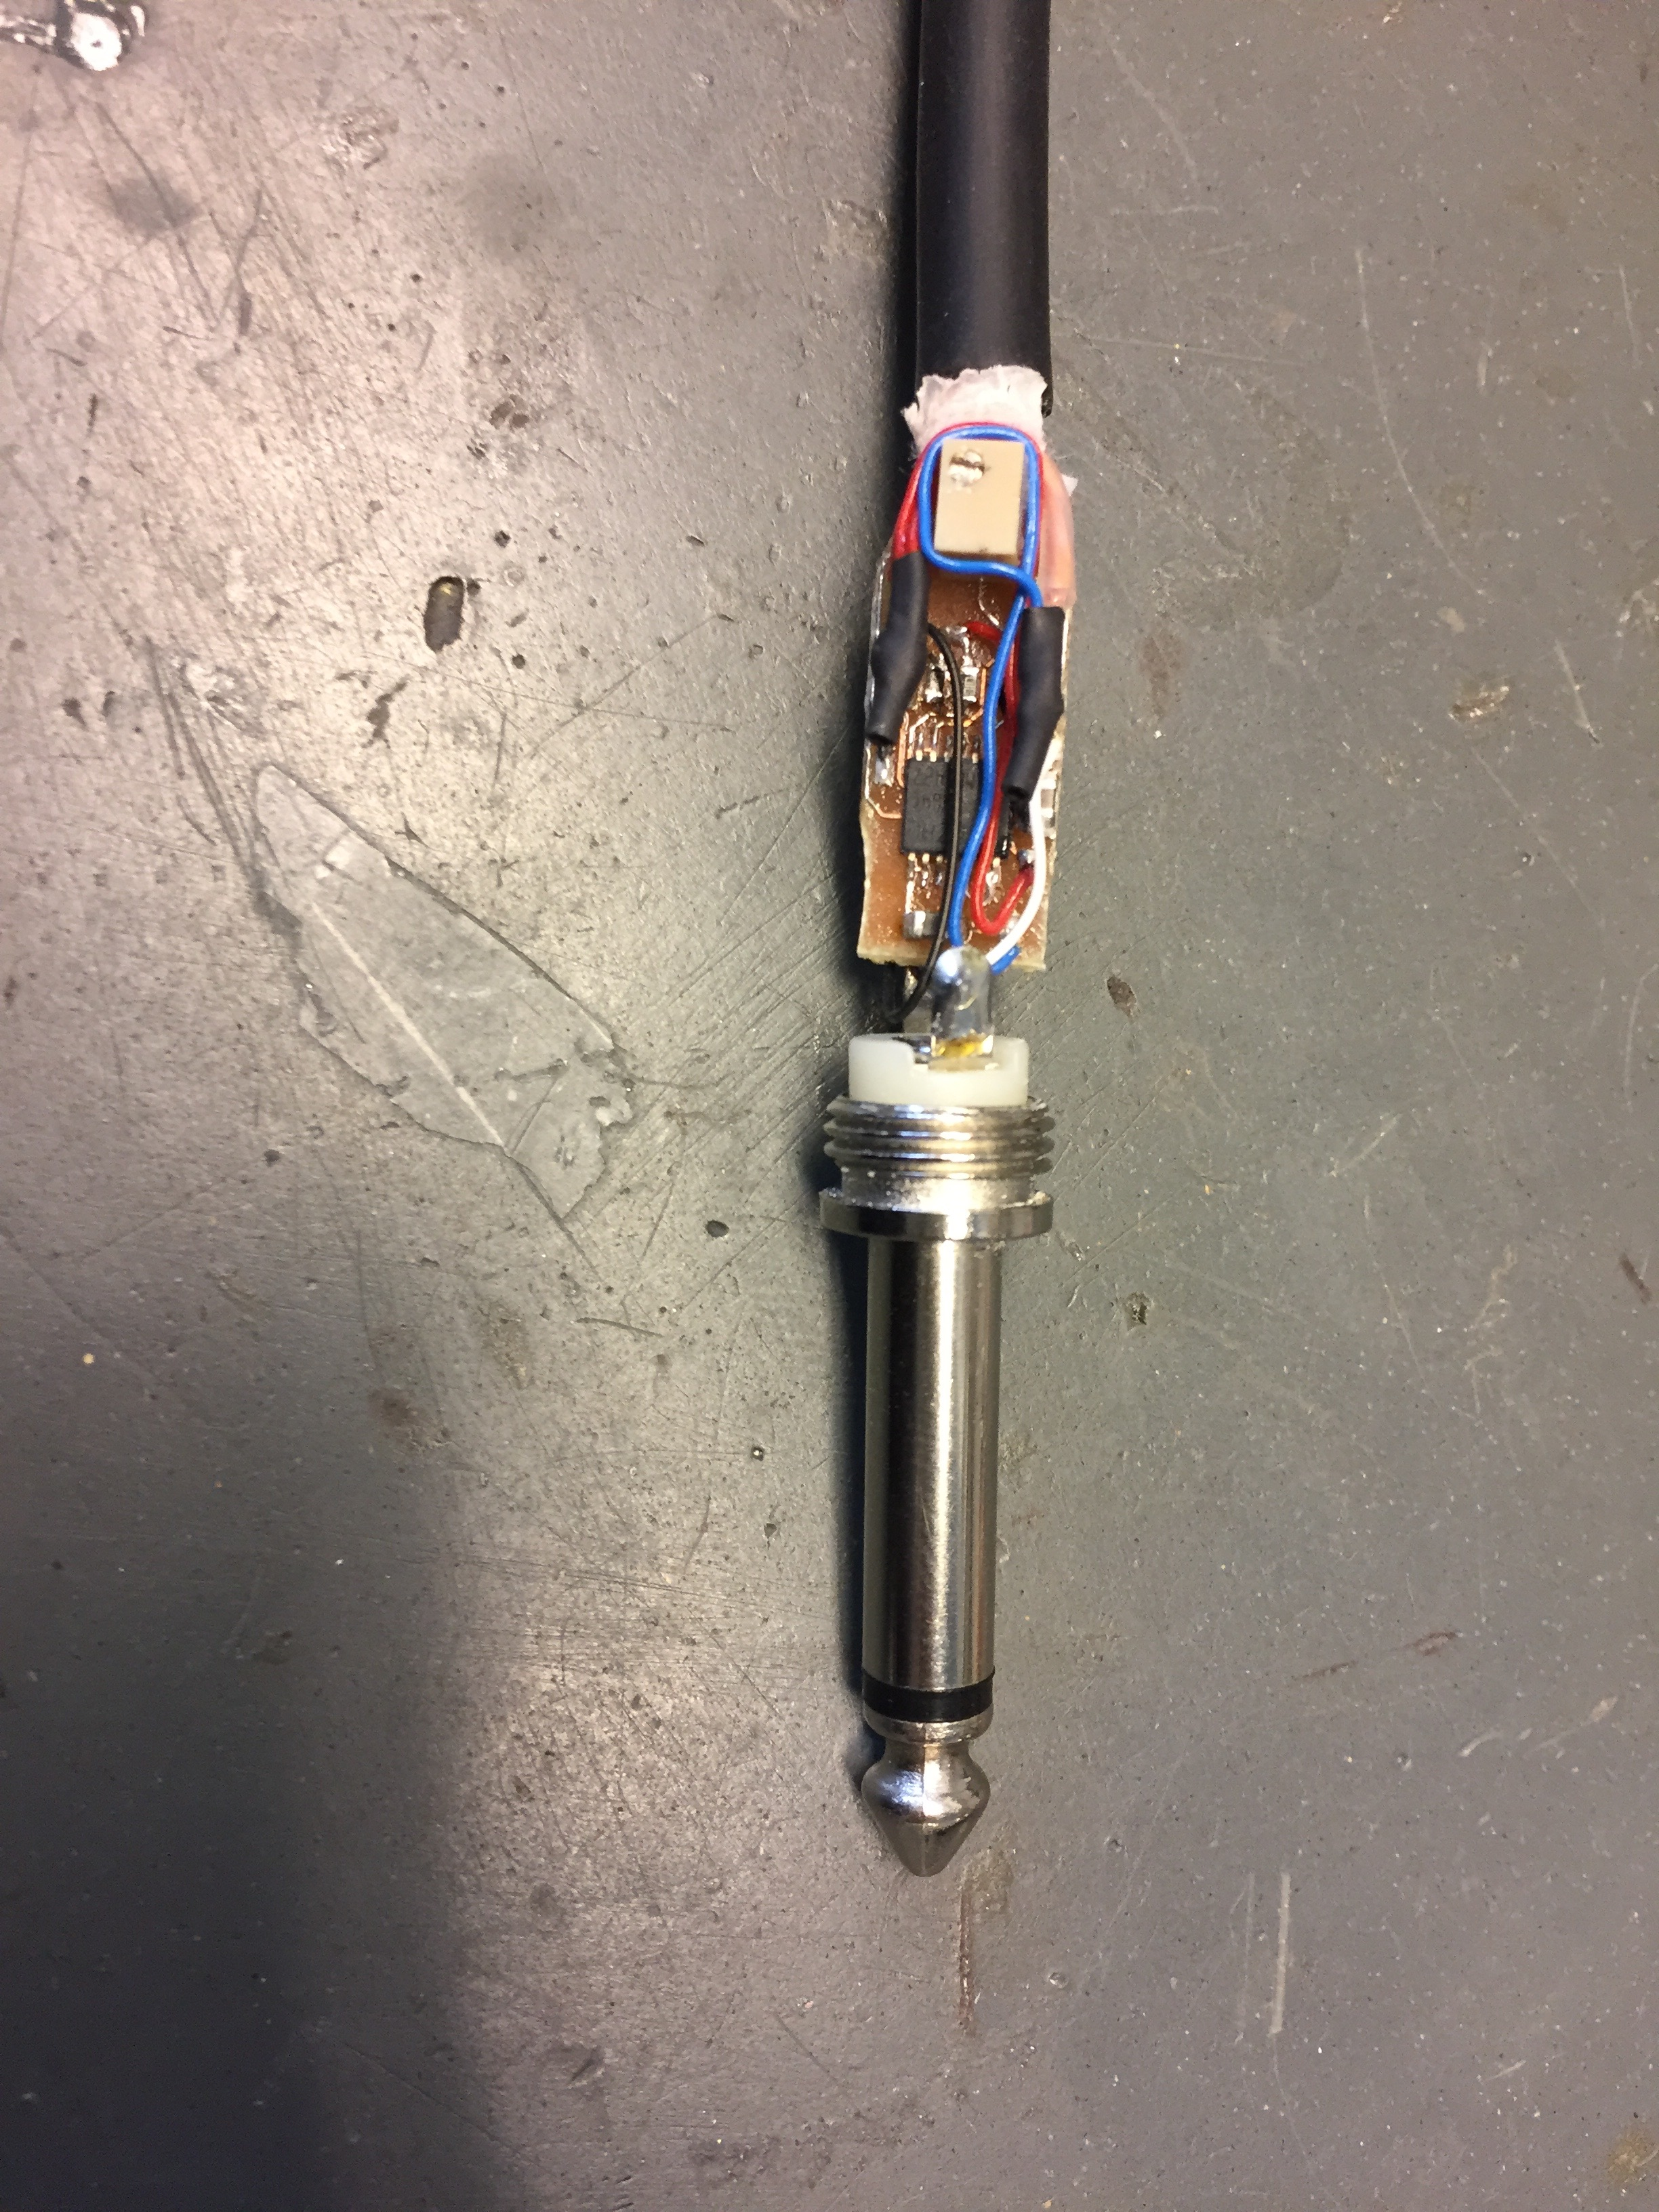
\includegraphics[width=0.4\textwidth , angle=90]{preamp_pcb.jpg}
		\caption{The picture shows the mounted \gls{preamp} \gls{pcb} }
		\label{fig:tests:preamp_pcb}
\end{figure} 

The second \autoref{fig:tests:preamp_jack} shows the \gls{preamp} \gls{pcb} mounted inside the jack connector house.

\begin{figure}[h]
	\centering
		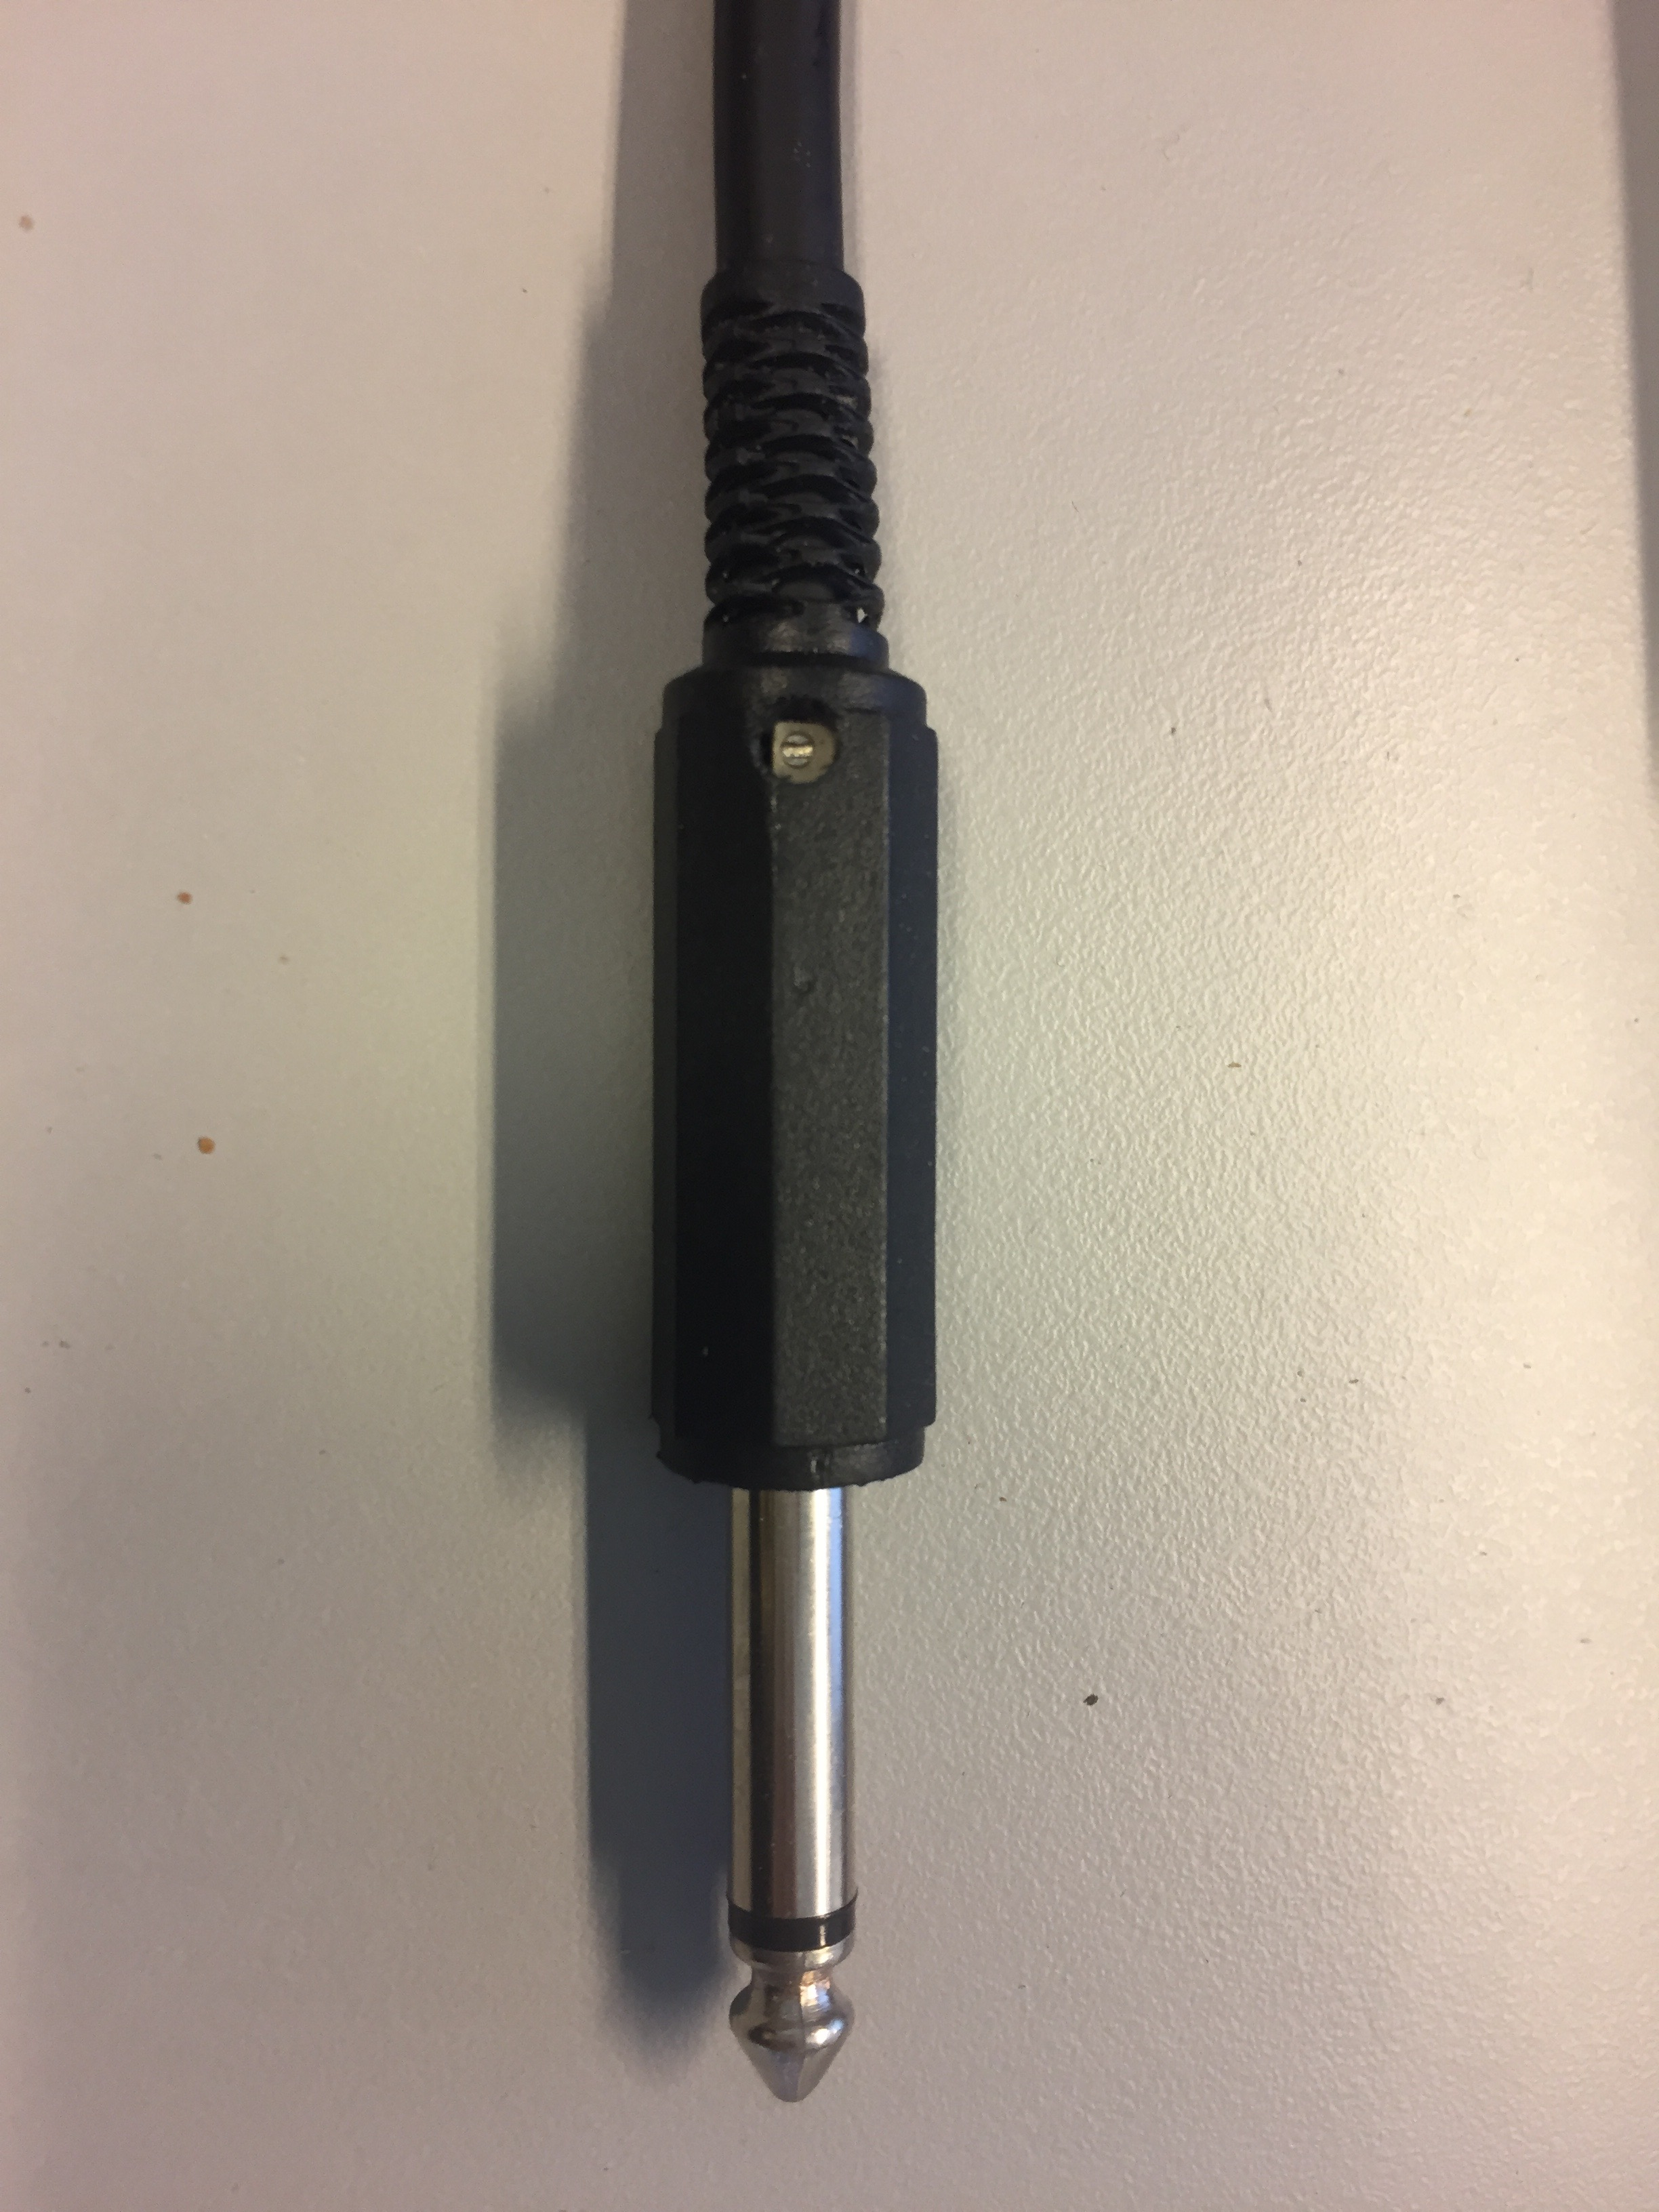
\includegraphics[width=0.4\textwidth , angle=90]{preamp_jack.jpg}
		\caption{The picture shows the mounted \gls{preamp} \gls{pcb} }
		\label{fig:tests:preamp_jack}
\end{figure} 

The \gls{preamp} \gls{pcb} fits inside the jack house, so \autoref{req:preamp5} and \autoref{req:preamp6} is approved